\chapter{Background}
\label{chap:background}

%\inspirationalquote{
%\begin{tabular}{p{0.83\textwidth}}
%Our society, our art, everything\inspirationalhyphen{}it's built on thousands of years of human innovation.
%So as long as you start on that foundation, and take it step by step\dots~you, too, can do amazing things.
%\end{tabular}}
%{Monika, Doki Doki Literature Club}

%\inspirationalquote{
%\begin{tabular}{p{0.83\textwidth}}
%I see now that none of us are yet ready. The cycle exists so that we may improve ourselves. But
%the one who reaches the summit is not our superior, for they stand on our shoulders to reach it.
%\end{tabular}}
%{The Shepherd v82.6.0174, The Talos Principle}

\inspirationalquote{We pray to our ancestors. We've met all of them. None of them were better than anyone else.}
{Mina, Iconoclasts}

This chapter will introduce the necessary background material on concurrency, stateless model checking, data-race analysis, and the relevant undergraduate operating systems classes.

\section{Concurrency}

\subsection{The Basics}

Modern software often turns to multithreading to improve performance.
In a multithreaded program, multiple execution units (or {\em threads}) execute the same or different sections of code simultaneously.
This can provide speedups up to a factor of the number of threads running in parallel,
but may also provide surprising execution results.

\subsubsection{Simultaneity}
This simultaneity of threads is achieved either by executing each one on a separate CPU, or by interleaving them nondeterministically (as controlled by clock interrupts) on the same CPU.
Because clock interrupts can occur at any instruction\footnote{
	With some exceptions in kernel-level programming, discussed later.
},
we consider single-CPU multithreading to be simultaneous at the granularity of individual instructions.
%
Likewise, when multiple CPUs access the same memory,
hardware protocols generally ensure that the events of a single instruction are executed atomically from the perspective of all CPUs.
Although there are some exceptions --
unlocked memory-to-memory instructions,
unaligned writes \cite{unaligned-writes},
and weak memory consistency models \cite{memory-consistency-models} --
we model multicore concurrency the same way as above,
deferring these exceptions beyond the scope of this work.
We refer to an execution trace depicting the global sequence of events as a {\em thread interleaving} or {\em schedule}.

\subsubsection{Shared state}
When a programming language offers multithreaded parallelism but forbids access to any shared state between threads \cite{rust-language},
the simultaneity of threads is largely irrelevant to the program's behaviour.
However, ``thread-unsafe'' languages such as C, C++, Java, and so on remain popular,
in which threads may access global or heap-allocated variables and data structures with no enforced access discipline.
The behaviour of such programs is then subject to the manner in which these accesses interleave.

\subsection{Identifying bugs}

Even if a program's behaviour is nondeterministic, that does not necessarily mean it has a bug.
After all, many programs use random number generation to intentionally generate different outputs.
We say a {\em concurrency bug} occurs when one or more of a program's nondeterministic behaviours is both {\em unanticipated} and {\em undesired}.
Most often, a concurrency novice who programs with shared state will consider the possible interleavings where one thread's access sequence occurs entirely before the other's, but neglect to consider intermediate outcomes in which the threads' access sequences are interleaved.

Consider the program in Figure \ref{fig:concurrency-bug}: Any output between 2 and 2000 is possible\footnote{
	Fun exercise for the reader: Show why 2 is a possible output, but 1 is not!
},
but whether this constitutes a bug is a matter of perspective.
Was the program written to count to 2000, or was it written to compute a randomized distribution?
In this thesis, we make no attempt to reason about the ``intent'' of programs,
so we further restrict {\em concurrency bug} to denote a program behaviour which is mechanically identifiable,
according to commonly-accepted notions of what programs behaviours are always bad.
%
Bug conditions include assertion failures,
memory access errors (i.e., segmentation fault or bus error),
heap errors (i.e., use-after-free or overflow),
deadlocks,
and infinite loops (which must be identified heuristically \cite{entscheidungsproblem}).

\begin{figure}[t]
	\begin{tabular}{cc}
		\begin{tabular}{p{0.45\textwidth}p{0.5\textwidth}}
			{\footnotesize
			\begin{tabular}{l}
				\texttt{int x;} \\
				\texttt{void count() \{} \\
				\texttt{~~~~for (int i = 0; i < 1000; i++)} \\
				\texttt{~~~~~~~~x++;} \\
				\texttt{\}} \\
				\texttt{void main() \{} \\
				\texttt{~~~~tid1 = thr\_create(count);} \\
				\texttt{~~~~tid2 = thr\_create(count);} \\
				\texttt{~~~~thr\_join(tid1);} \\
				\texttt{~~~~thr\_join(tid2);} \\
				\texttt{~~~~printf("\%d\textbackslash{}n", x);} \\
				\texttt{\}} \\
			\end{tabular}
			}
			&
			{\footnotesize \begin{tabular}{ll}
				{\bf \normalsize Thread 1} & {\bf \normalsize Thread 2} \\
				\hline
				\texttt{load tmp <- x;} & \\
				& \texttt{load tmp <- x;} \\
				& \texttt{add tmp <- 1;} \\
				& \texttt{store x <- tmp;} \\
				\texttt{add tmp <- 1;} & \\
				\texttt{store x <- tmp;} & \\
			\end{tabular}
			}
			\\
			\\
			(a) Source listing for a multithreaded program which might count to 2000.
			&
			(b) Example interleaving of the compiled assembly for (a),
			in which 2 concurrent iterations of the loop yield 1 net increment of {\tt x}.
		\end{tabular}
	\end{tabular}
	\caption{Example concurrent program in which simultaneous accesses to shared state may interleave to produce unexpected results.}
	\label{fig:concurrency-bug}
\end{figure}

\subsection{Concurrency Primitives}

To prevent unexpected interleavings such as the example in Figure~\ref{fig:concurrency-bug}(b),
most concurrent programs use {\em concurrency primitives} to control which interleavings are possible.
Controlling nondeterminism is not typically provided by any features of programming languages themselves;
rather, it is achieved via special atomicity mechanisms provided by the CPU and/or operating system -- hence the term ``primitive''.
For example, x86 CPUs provide the {\tt xchg} instruction, which performs both a read and subsequent write to some shared memory, with no possibility for other logic to interleave in between.
Using such atomic instructions as building blocks, concurrency libraries provide abstractions for controlling nondeterminism in several commonly-desired ways.
These include {\em locks}, {\em descheduling}, {\em condition variables}, {\em semaphores}, {\em reader-writer locks}, and {\em message-passing}.

\begin{figure}[t]
	\begin{tabular}{p{0.45\textwidth}p{0.5\textwidth}}
		{\footnotesize
		\begin{tabular}{l}
			\texttt{typedef struct mutex \{} \\
			\texttt{~~~~volatile int held;} \\
			\texttt{~~~~int owner;} \\
			\texttt{\} mutex\_t;} \\
			\texttt{void mutex\_lock(mutex\_t *mp) \{}\\
			\texttt{~~~~while (xchg(mp->held, 1))} \\
			\texttt{~~~~~~~~yield(mp->owner);} \\
			\texttt{~~~~mp->owner = gettid();} \\
			\texttt{\}} \\
			\texttt{void mutex\_unlock(mutex\_t *mp) \{}\\
			\texttt{~~~~mp->owner = -1;} \\
			\texttt{~~~~mp->held = 0;} \\
			\texttt{\}} \\
		\end{tabular}
		}
		&
		{\footnotesize
		\begin{tabular}{l}
			\texttt{int x;} \\
			\texttt{mutex\_t m;} \\
			\texttt{void count() \{} \\
			\texttt{~~~~for (int i = 0; i < 1000; i++) \{} \\
			\texttt{~~~~~~~~mutex\_lock(\&m);} \\
			\texttt{~~~~~~~~x++;} \\
			\texttt{~~~~~~~~mutex\_unlock(\&m);} \\
			\texttt{~~~~\}} \\
			\texttt{\}} \\
		\end{tabular}
		}
		\\
		(a) A simple mutual exclusion lock built using the {\tt xchg} instruction. %(accessed using a GCC compiler intrinsic).
		&
		(b) The {\tt count} function from Figure~\ref{fig:concurrency-bug}, adjusted to use a mutex to ensure each increment of {\tt x} is uninterruptible.
	\end{tabular}
	\caption{Using a locking primitive to protect accesses to shared state.}
	\label{fig:mutex}
\end{figure}

Each such abstraction provides certain semantics about what thread interleavings can arise surrounding their use.
When building a tool for testing concurrent programs,
one may include some computational understanding of the behaviour of any, or all, of these abstractions.
Annotating a certain abstraction's semantics treats it as a trusted concurrency primitive in its own right,
and allows the testing tool to reduce the possible space of interleavings (or the set of false positive data-race candidates reported, etc.),
at the cost of increasing the implementation and theoretical complexity of the analysis.
This thesis will consider locks, descheduling, and transaction begin/end as the only concurrency primitives,
and assume the others listed above are implemented using those as building blocks (an exercise for the reader \cite{thrlib}).

Locks (or {\em mutexes}, short for ``mutual exclusion locks'') are objects, shared by multiple threads, which allow the programmer to mark certain {\em critical sections} of code that must not interleave with each other.
When one thread completes a call to {\tt mutex\_lock(mp)}, all invocations by other threads on the same {\tt mp} will wait (or ``block'') until the corresponding {\tt mutex\_unlock(mp)}.
Figure~\ref{fig:mutex}(a) shows how a yielding mutex (not the best implementation, but the simplest) may be implemented using {\tt xchg},
and (b) shows how a mutex may be used to fix the example from Figure~\ref{fig:concurrency-bug}.


\subsection{Transactional Memory}
\label{sec:overview-tm}

Critical sections of code must be protected from concurrent access, even when it's not known in advance whether the shared memory accesses between threads will actually conflict on the same memory addresses.
The concurrency primitives discussed above take a pessimistic approach, imposing a uniform performance penalty (associated with the primitives' implementation logic) on all critical sections, whether or not a conflict is likely.
Some implementations may be optimized for ``fast paths'' in the absence of contention, but must still access shared memory in which the primitive's state resides.

Transactional memory \cite{transactional-memory} offers a more optimistic approach: critical sections of code are marked as ``transactions'', analogously to locking a mutex, and allowed to speculatively execute with no protection.
If a conflict between transactions is detected, the program state is rolled back to the beginning of the transaction, and a backup code path may optionally be taken.
Consequently, no intermediate state of a transacting thread is ever visible to other threads; all changes to memory within a transaction become globally visible ``all at once'' (or not at all).
This method optimizes for a common no-contention case of little-to-no overhead, pushing extra both code and implementation complexity to handling conflicts.

Transactional memory (TM) may be implemented either in hardware, using special instructions and existing cache coherence algorithms,
or in software, via library calls and a log-based commit approach.
Software transactions (STM) \cite{stm-pldi06} can be used on any commodity processor, but must impose runtime overhead associated with logging.
Hardware transactions (HTM) \cite{intel-tsx-overview}
%\cite{htm-experience, htm-performance}
achieve better performance by reusing existing cache coherence logic to detect conflicts, but require explicit support from the CPU, which is not yet widespread.
Haswell \cite{htm-haswell} is the first x86 architecture to support HTM,
offering three new instructions: \texttt{xbegin}, \texttt{xend}, and \texttt{xabort}, to begin, commit, and fail a transaction, respectively.
The example program in Figure~\ref{fig:htm-example} demonstrates how these primitives can be used to synchronize a simple shared access without locking overhead in the common case\footnote{
	The solution presented here is actually incomplete; stay tuned until Chapter~\ref{chap:tm} for the surprising twist!
},
using GCC's compiler intrinsics \cite{htm-gcc}.

\begin{figure}[h]
	\begin{center}
		\begin{tabular}{l}
		\texttt{\ctype{void} \call{count}() \{} \\
		\texttt{~~~~\flow{for} (\ctype{int} i = \const{0}; i < \const{1000}; i++) \{} \\
		\texttt{~~~~~~~~\flow{if} ((status = \call{\_xbegin}()) == \const{\_XBEGIN\_STARTED}) \{} \\
		\texttt{~~~~~~~~~~~~x++;} \\
		\texttt{~~~~~~~~~~~~\call{\_xend}();} \\
		\texttt{~~~~~~~~\} \flow{else} \{} \\
		\texttt{~~~~~~~~~~~~\call{mutex\_lock}(\&m);} \\
		\texttt{~~~~~~~~~~~~x++;} \\
		\texttt{~~~~~~~~~~~~\call{mutex\_unlock}(\&m);} \\
		\texttt{~~~~~~~~\}} \\
		\texttt{~~~~\}} \\
		\texttt{\}} \\
		\end{tabular}
	\end{center}
	\caption{The example {\tt count} routine from Figure~\ref{fig:mutex}, rewritten to use HTM.
		If the transaction in the top branch aborts,
		whether from a memory conflict or random system interrupt,
		%from the programmer's intention,
		execution will revert to the return of {\tt \_xbegin},
		{\tt status} will be assigned an error code indicating the abort reason,
		and control will drop into the {\tt else} branch.
		The programmer can then use explicit synchronization, such as a mutex, to resolve the conflict.}
	\label{fig:htm-example}
\end{figure}

Concerning possible execution patterns,
the main difference between STM and HTM is the circumstances under which a transaction may abort.
A software-backed transaction will abort if and only if a memory conflict occurs therein with another thread.
HTM, however, is backed by the CPU's cache, and is therefore subject to other circumstances such as cache capacity or interrupt-triggered cache flushes which may force an abort even when no memory conflict occurs.
Chapter~\ref{chap:tm} will explore the consequences of this difference further.
%
This thesis will focus on HTM as my platform for testing transactional programs,
to highlight the importance of researching advanced testing techniques in anticipation of upcoming hardware features.

%%%%%%%%%%%%%%%%%%%%%%%%%%%%%%%%%%%%%%%%%%%%%%%%%%%%%%%%%%%%%%%%%%%%%%%%%%%%%%%%

\section{Stateless Model Checking}
\label{sec:overview-stateless} % ugh this label name

Model checking \cite{verisoft} is a testing technique for systematically exploring the possible thread interleavings of a concurrent program.
A model checker executes the program repeatedly, each time according to a new thread interleaving, until all interleavings have been tested or the CPU budget is exhausted.
During each execution, it forces threads to execute serially, thereby confining the program's nondeterminism to scheduler thread switches.
It then controls the scheduling decisions
%, choosing a different thread from one chosen before at a certain execution states
to guarantee a unique interleaving is tested each iteration.

\subsection{The state space}

To understand what it means to exhaustively test all possible thread interleavings,
one must define the possible execution sequences as a finite {\em state space}.
To visualize this,
using a single iteration of the {\tt x++;} loop from Figure~\ref{fig:concurrency-bug} as an example,
with {\tt x++;} expanded into its three corresponding pseudo-assembly instructions,
Figure~\ref{fig:tree}(a) shows all possible execution interleavings
%of the compiled code
between 2 threads.

\begin{figure}[p]
	\begin{tabular}{c}
		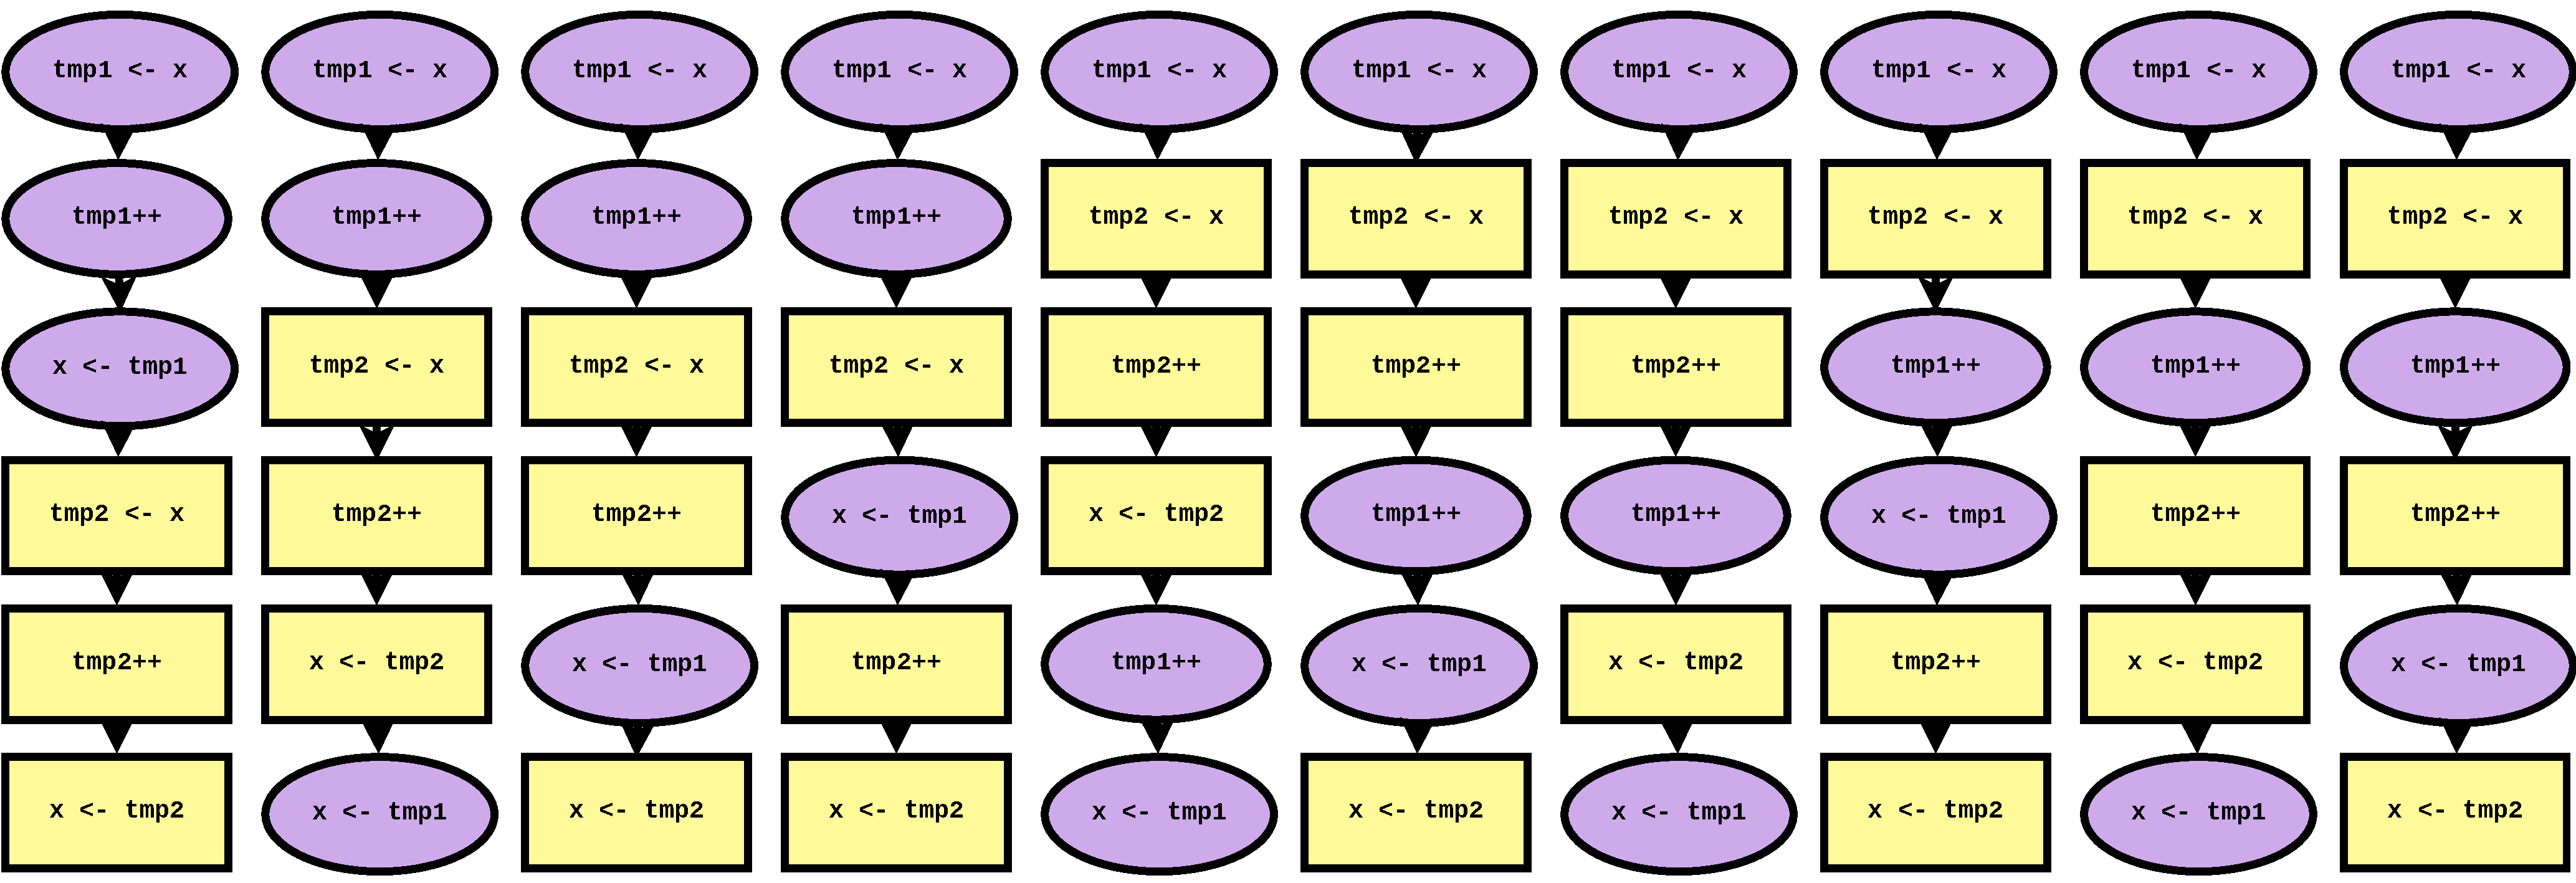
\includegraphics[width=\textwidth]{statespace-list.pdf}
		\\
		(a) Interleavings visualized individually, as a list.
		\\
		\\
		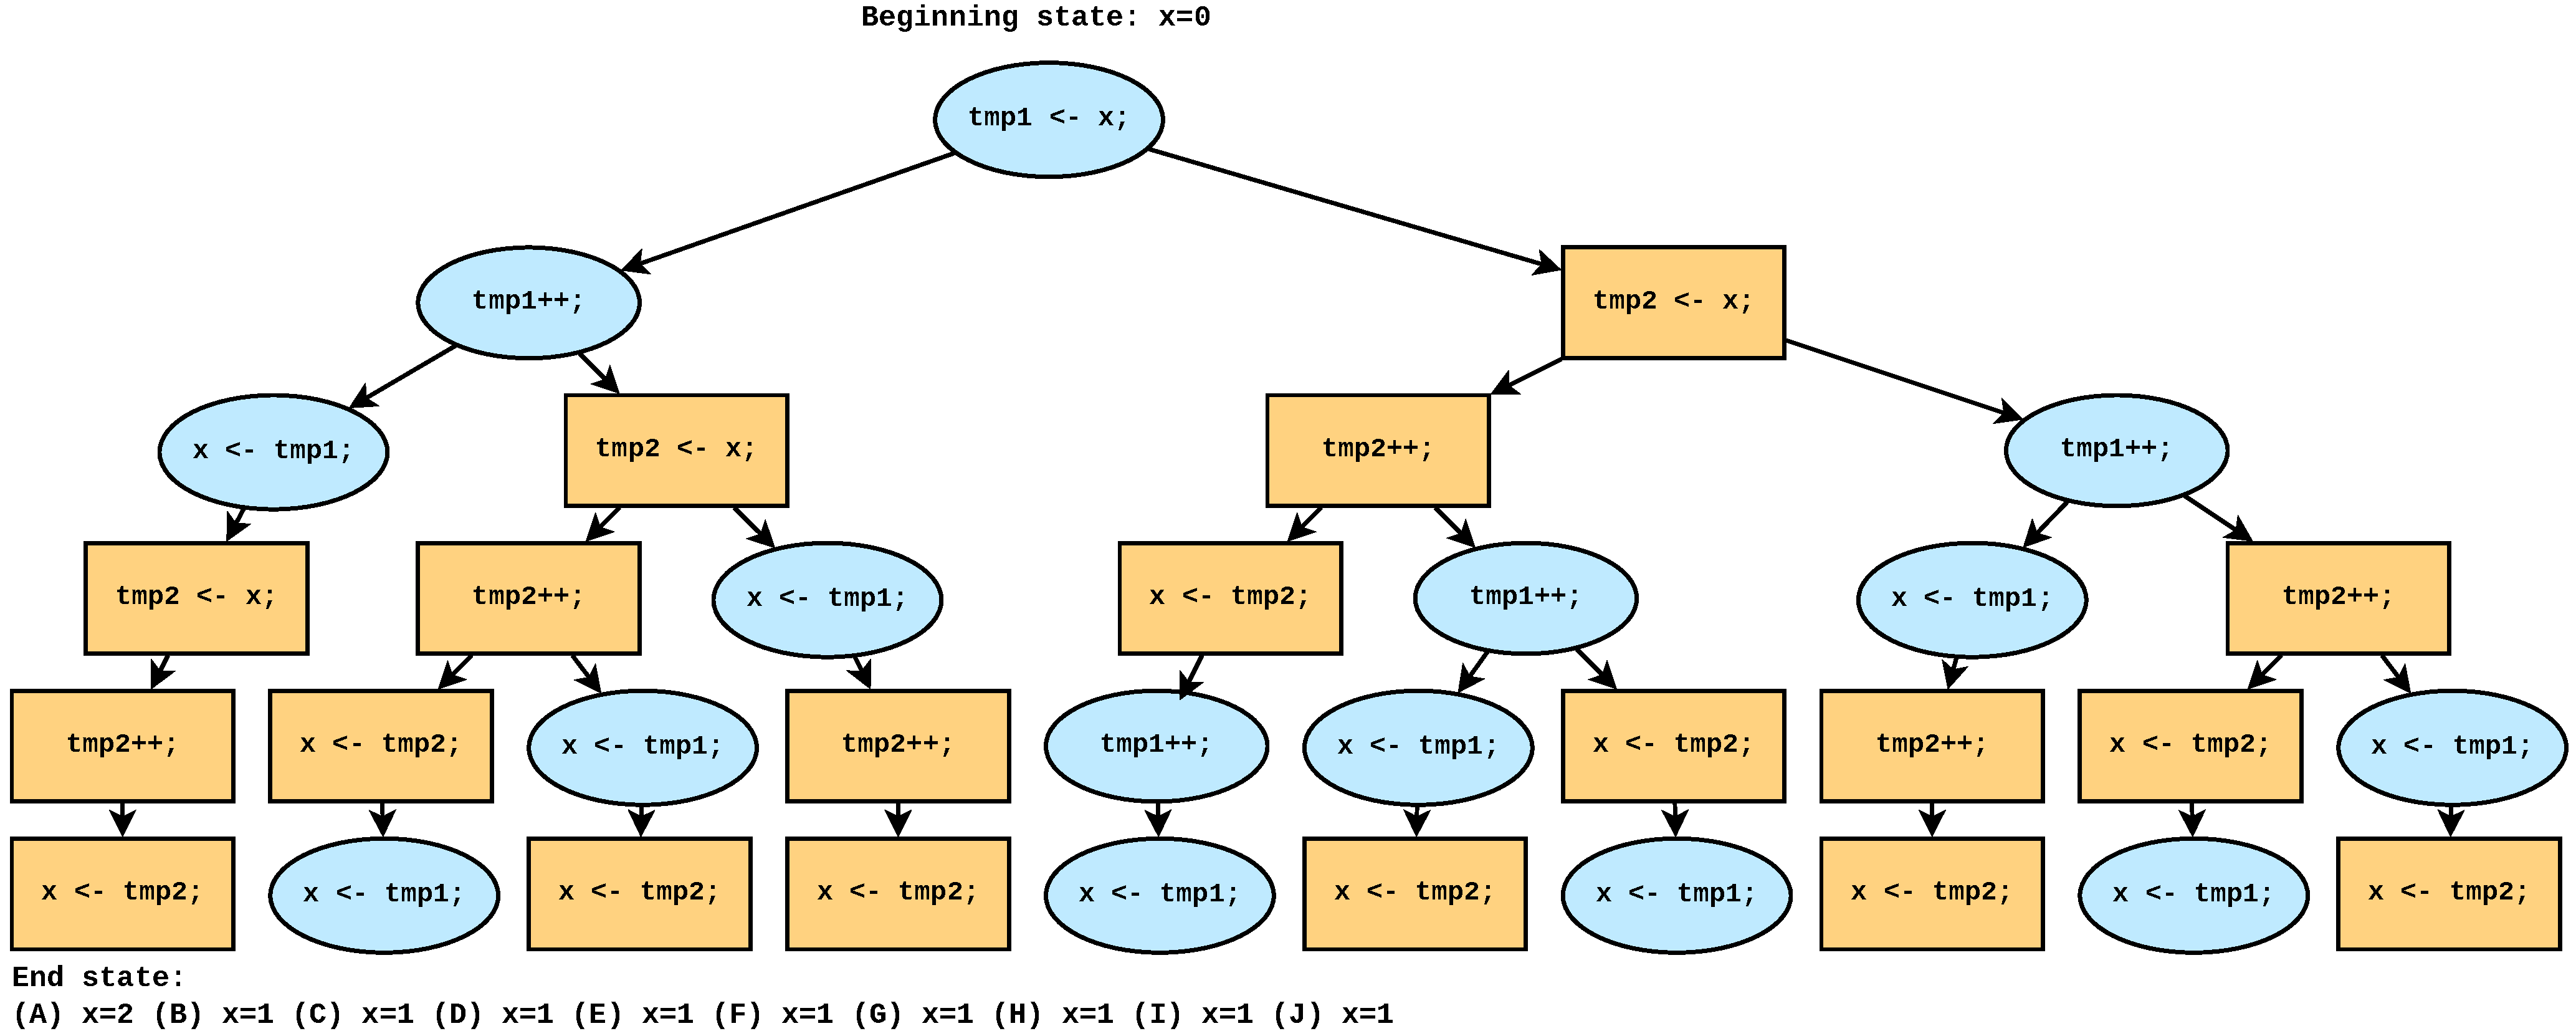
\includegraphics[width=\textwidth]{statespace-tree.pdf}
		\\
		(b) Interleavings (same order as in (a)), with common prefixes \\
		combined as ``preemption points'', forming a tree.
	\end{tabular}
	\caption{Visualization of interleaving state space for the program in Figure~\ref{fig:concurrency-bug}.
	Thread 1 is represented by purple ovals, thread 2 by yellow squares, and time flows from top to bottom.
	As the two threads execute the same code, without loss of generality thread 1 is fixed to run first --
	the full state space is twice the size, and the other half is symmetric to the one shown.}
	\label{fig:tree}
\end{figure}

\subsubsection{Static versus dynamic analysis}

Model checking is a {\em dynamic} program analysis, meaning that it observes the operations and accesses performed by the program as its code is executed.
In contrast, {\em static} program analyses check certain properties at the source code level.
Static analyses are ideal for ensuring certain standards of code quality, which often correlates with correctness,
but cannot decide for certain whether a given program will fail during execution without actually running the code \cite{incompleteness}.
Static analyses face the challenge of {\em false alarms} (or {\em false positives}):
code patterns which look suspicious but are actually correct.
A debugging tool which reports too many false alarms will dissuade developers from using it \cite{racerx}.
Dynamic analysis, our approach, identifies program behaviours that are definitely wrong,
so each bug report is accompanied by concrete evidence of the violation.
Assertions, segfaults, use-after-free of heap memory, and deadlock are examples of such failures we check for,
although a checker may also include arbitrary program-specific predicates.

\subsubsection{Preemption points}

During execution, a model checker identifies a subset of the program's operations as ``interesting'', i.e.,
where interrupting the current thread to run a different one is likely to produce different behaviour.
These so-called {\em preemption points} may be identified by any combination of human intuition and machine analysis.
Typical preemption points include the boundaries of synchronization APIs (e.g., {\tt mutex\_lock}) or accesses to shared variables.
Considering that at each preemption point multiple threads exist as options to run next,
the set of possible ways to execute the program can be viewed as a tree.
Figure~\ref{fig:tree}(b) shows a visualization of the corresponding tree from our example program,
using each pseudo-assembly instruction as a preemption point.

The number of preemption points in each execution defines the depth of this tree,
and the number of threads available to run defines the branching factor.
Hence, in a program with $n$ preemption points and $k$ threads available to run at each, the state space size is $O(n^k)$.
Nevertheless, to fully test all of a program's possible behaviours, we must check the executions corresponding to every branch of the tree.
Addressing the scaling problem in this exponential relation is the central research problem for all model checkers.

Some model checkers explicitly store the set of visited program states as a means of identifying equivalent interleavings \cite{spin}.
From the perspective of such tools, state spaces such as these wherein equivalent states may be reached by multiple paths
are represented as a directed acyclic graph (DAG) instead of as a tree.
This approach is called {\em stateful} model checking.
This thesis focuses on {\em stateless} model checking (and execution trees, not DAGs),
which instead analyzes the sequence of execution events to avoid a prohibitive memory footprint.
Henceforth ``stateless model checking'' will be abbreviated simply as ``model checking'' for brevity.
Also, the term ``state space'' was originally coined to refer to the stateful approach's emphasis on the DAG's nodes
(i.e., program states);
while stateless checkers emphasize the tree's branches (i.e., execution sequences) instead,
I will continue to use ``state space'' for consistency with prior work.

\subsection{On the size of state spaces}

At its essence, stateless model checking research is a perpetual struggle to become more and more efficient in order to test and verify bigger and bigger programs.
But whence this efficiency?
Techniques for coping with the exponential explosion fall into two categories:
(1) removing redundant interleavings from the state space when we can prove they are equivalent to some interleaving already tested,
or {\bf reduction techniques},
and
(2) prioritizing interleavings judged as more likely to contain bugs should bugs exist
in case we are unable to exhaustively test all interleavings after all,
or {\bf search heuristics}.

\subsubsection{Reduction techniques}

Dynamic Partial Order Reduction \cite{dpor} (henceforth, DPOR) is the most popular algorithm for mitigating the exponential explosion that arises as program size increases.

{\bf Abstractly speaking:}
Let {\em independent transitions} denote a pair of executions of two threads, each from one preemption point to the next,
in which there are no read/write or write/write access pairs to the same memory between threads.
DPOR reduces a state space, originally exponentially-sized in the number of thread transitions,
to an equivalent one
(i.e., testing which suffices to check all program behaviours that could arise in the original state space)
exponentially-sized in the number of {\em dependent} thread transitions.
%More intuitively, if two thread transitions between preemption points do not conflict on any shared resource access,
%reordering them produces an equivalent interleaving, i.e., the same program behaviour.
More technically, it identifies equivalent execution sequences according to Mazurkiewicz trace theory \cite{mazurkiewicz},
and tests at least one execution from each equivalence class.

{\bf Concretely speaking:}
Figure~\ref{fig:dpor} highlights part of an execution tree where the execution ordering of threads 1 and 2 are swapped,
and each interleaving has a respective ``subtree'' (i.e., possible interleavings given the fixed execution prefix leading up to it).
The specifics of execution before the thread 1/thread 2 sequence,
other possible threads to run instead of threads 1 or 2,
and what logic the program executes in those subtrees
are all presumably arbitrary.
In these two highlighted branches,
if the transitions of threads 1 and 2 are {\em independent},
%if the operations performed by threads 1 and 2 are independent
%(i.e., no write/read or write/write access pairs to the same memory),
DPOR deduces that the subsequent program states (indicated by the red arrow) are equivalent.
Thence, only one of the two interleavings and its respective subtree needs to be executed
in order to check all possible program states.
\sect{\ref{sec:landslide-dpor}} explains how DPOR implements such a deduction in more detail.

Over the years, researchers have developed many enhancements to DPOR, such as Optimal DPOR \cite{optimal-dpor}, parallelizable DPOR \cite{parallel-dpor}, SAT-directed model checking \cite{satcheck}, Maximal Causality Reduction \cite{mcr}, and DPOR for relaxed memory architectures \cite{tsopso}.

\begin{figure}[t]
	\begin{center}
	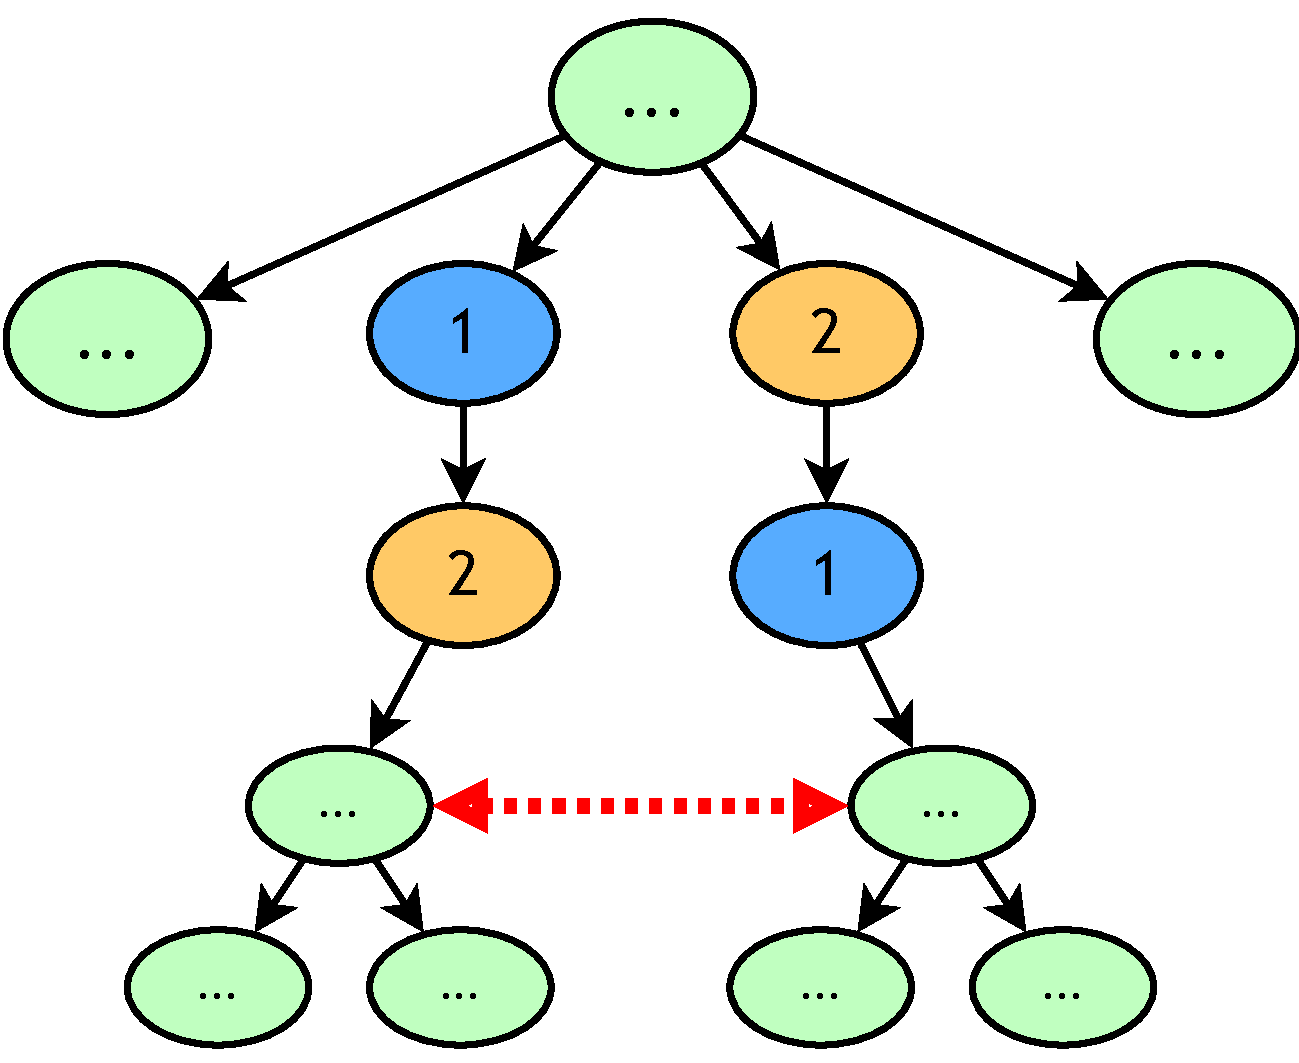
\includegraphics[width=0.4\textwidth]{dpor.pdf}
	\end{center}
	\caption{DPOR identifies independent transitions by different threads which can commute without affecting program behaviour. Here, if the transitions marked 1 and 2 have no shared memory conflicts, the states marked with the red arrow are guaranteed identical. Hence, only one of the subtrees need be explored.}
	\label{fig:dpor}
\end{figure}

\subsubsection{Search heuristics}

However, even though DPOR can prune an exponential number of redundant interleavings, the state space size is still exponential in the number of {\em dependent} (conflicting) interleavings.
Developers will always want to test larger and larger programs, so no matter the quality of our reduction algorithm,
we must accept that some tests will be too large to be fully tested in a reasonable time.
Hence, recent model checking research has turned to heuristic techniques for achieving further reduction,
optimizing the search to try to uncover bugs faster (should they exist)
at the expense of possibly missing other bugs,
or missing the chance to complete a full verification.

Iterative Context Bounding \cite{chess-icb} is a popular such technique which heuristically reorders the search to prioritize interleavings with fewer preemptions first.
This heuristic is based on the insight that most bugs require few preemptions to uncover, so interleavings with a number of preemptions that exceeds a certain bound will be de-prioritized, only tested until after all the fewer-preemption interleavings are completed.
Preemption sealing \cite{sealing} is another heuristic strategy which restricts the scope of the search by limiting the model checker to use only preemption points arising from certain functions in the source code.
This allows developers to vastly reduce state space size by identifying which program modules are already trusted,
although it requires some human intuition to correctly mark those boundaries.
Iterative Deepening, presented in Chapter~\ref{chap:quicksand}, is another such search heuristic.

%%%%%%%%%%%%%%%%%%%%%%%%%%%%%%%%%%%%%%%%%%%%%%%%%%%%%%%%%%%%%%%%%%%%%%%%%%%%%%%%

\section{Data Race Analysis}
\label{sec:background-datarace}

\begin{figure}[t]
        \small
	\begin{center}
\begin{tabular}{c}
\begin{tabular}{rll}
        & \multicolumn{2}{c}{\texttt{int x = 0; bool y = false; mutex\_t mx;}} \\
        \\
        & {\bf Thread 1} & {\bf Thread 2} \\
        1 & \texttt{\hilight{brickred}{x++;}~// A1} & \\
        2 & \texttt{mutex\_lock(\&mx);} & \\
        3 & \texttt{mutex\_unlock(\&mx);} & \\
        4 & & \texttt{mutex\_lock(\&mx);} \\
        5 & & \texttt{mutex\_unlock(\&mx);} \\
        6 & & \texttt{\hilight{brickred}{x++;}~// A2} \\
\end{tabular}
\\
\\
	{\normalsize (a) True potential data race.}
\\
\\
\begin{tabular}{rll}
        %& \multicolumn{2}{c}{\texttt{int x = 0; bool y = false; mutex\_t mx;}} \\
        & {\bf Thread 1} & {\bf Thread 2} \\
        1 & \texttt{\hilight{brickred}{x++;}~// B1} & \\
        2 & \texttt{mutex\_lock(\&mx);} & \\
        3 & \texttt{y = true;} & \\
        4 & \texttt{mutex\_unlock(\&mx);} & \\
        5 & & \texttt{mutex\_lock(\&mx);} \\
        6 & & \texttt{bool tmp = y;} \\
        7 & & \texttt{mutex\_unlock(\&mx);} \\
        8 & & \texttt{if (tmp) \hilight{brickred}{x++;}~// B2} \\
        %8 & & \texttt{if (tmp)} \\
        %9 & & \texttt{~~~~\hilight{brickred}{x++;}~// B2} \\
\end{tabular}
\\
\\
{\normalsize (b) No data race in any interleaving.}
\end{tabular}
	\end{center}
\caption{{Data-race analyses may be prone to either {\em false negatives} or {\em false positives}.
Applying Happens-Before to program (a) will miss the potential race possible between A1/A2 in an alternate interleaving,
while using Limited Happens-Before on (b) will produce a false alarm on B1/B2.}}
\label{fig:hb-example}
\end{figure}

\subsection{Definition}

Data race analysis \cite{eraser} identifies pairs of unsynchronized memory accesses between threads.
Two instructions are said to race if:
\begin{enumerate}
	\item they both access the same memory address,
	\item at least one is a write,
	\item the threads do not hold the same lock,
	\item and no synchronization enforces an order on the thread transitions (the {\em Happens-Before} relation, described below).
\end{enumerate}
%In Figure~\ref{fig:example}, lines 3 and 5 each race with 2 and 6, and line 6 races with 8.
In Figure~\ref{fig:hb-example}, the pairs of lines marked with comments (A1 and A2, B1 and B2) race.

A data race analysis may be either {\em static} (inspecting source code) \cite{racerx} or {\em dynamic} (tracking individual accesses arising at run-time) \cite{tsan}.
This paper focuses exclusively on dynamic analysis,
so although our example refers to numbered source lines for ease of explanation,
in practice we are actually classifying the individual memory access events corresponding to those lines during execution.
Actually, each {\tt x++} statement likely compiles to two separate load or store instructions, so each of those two instructions from each of the two marked source lines pairwise will race (except for the two loads, which are both reads).

\subsection{Happens-Before}
\label{sec:background-hb}

Condition 4 of the above definition expresses the notion that the access pair can be executed concurrently,
regardless of whether the hardware actually carries out the operations in the same physical instant.
Several approaches exist to formally representing this condition.

\begin{itemize}
	\item Most prior work focuses on {\em Happens-Before} \cite{lamport-clocks} as the order relation between accesses.
\cite{predictive-dr} and \cite{hybriddatarace} identify a problem with this approach:
it cannot identify access pairs separated by an unrelated lock operation which could race in an alternate interleaving,
as shown in the example program in Figure~\ref{fig:hb-example}(a).
We call such unreported access pairs {\em false negatives}.

\item
\cite{hybriddatarace} introduces the {\em Limited Happens-Before} relation,
which will report such potential races
by considering only blocking operations like {\tt cond\_wait} to enforce the order.
However, consider the similar program in Figure~\ref{fig:hb-example}(b),
in which the access pair ceases to exist in the alternate interleaving.
Limited Happens-Before will report all potential races, avoiding false negatives \cite{tsan},
but at the cost of necessarily reporting some such {\em false positives}.

\item
In recent work, the {\em Causally-Precedes} relation \cite{predictive-dr} %strikes a middle ground,
extends Happens-Before to additionally report a subset of potential races while soundly avoiding false positives.
It tracks conflicting accesses in intervening
critical sections to determine whether lock events are unrelated to a potential race.
Causally-Precedes will identify the potential race in Figure~\ref{fig:hb-example}(a), as the two critical sections do not conflict,
although it can still miss true potential races in other cases.
\end{itemize}

Landslide implements both Happens-Before (henceforth referred to as {\em Pure Happens-Before} for clarity) and Limited Happens-Before.
Chapter~\ref{chap:quicksand} includes a comparison of the two approaches for the purpose of finding new preemption points for model checking.
%, we use the Limited Happens-Before relation for our analysis.
%The justification for this is that, while stand-alone data-race analyses must avoid inundating the user with false alarms \cite{racerx},
%my work incorporates data-race analysis in an internal feedback loop, and reports only directly observed failures to the user.
%Hence, I accept some overhead from false positives for the sake of more thorough testing.

%%%%%%%%%%%%%%%%%%%%%%%%%%%%%%%%%%%%%%%%%%%%%%%%%%%%%%%%%%%%%%%%%%%%%%%%%%%%%%%%

\section{Education}
\label{sec:overview-edu}

This thesis will tackle Pebbles and Pintos, two different system architectures used in educational operating systems courses.
This section describes the projects which students implement and which Landslide tests.

\subsection{Pebbles}
\label{sec:pebbles}

The Pebbles kernel architecture
is used at Carnegie Mellon University (CMU) in 15-410, Operating System Design and Education \cite{kspec,thrlib}.
In the course of a semester, students work on five programming assignments;
the first two are individual, and the remaining three are the products of two-person teams.
I will focus on the third and fourth of these, the thread library and kernel,
called ``P2'' and ``P3'' respectively (the project numbers start at 0).
The other three (a stack-crawling backtrace utility, a bare-metal game with device drivers, and a small extension to the P3 kernel) are not of concern in this thesis.
The course's prerequisite is 15-213, Introduction to Computer Systems \cite{sigcse01:CSaPP}.
Both P2 and P3 are built using the {\em Pebbles} system call specification, outlined in Table~\ref{tab:syscalls}

\begin{table}
        \center
        \begin{tabular}{|l|p{0.75\textwidth}|}
                \hline
                \bf System call name & \bf Summary \\
                \hline
                \multicolumn{2}{c}{\em Lifecycle management} \\
                \hline
                \texttt{fork} & Duplicates the invoking task, including all memory regions. \\
                \texttt{thread\_fork} & Creates a new thread in the current task.\\
                \texttt{exec} & Replaces the program currently running in the invoking task with a new one specified. \\
                \texttt{set\_status} & Records the exit status of the current task. \\
                \texttt{vanish} & Terminates execution of the calling thread. \\
                \texttt{wait} & Blocks execution until another task terminates, and collects its exit status.\\
                \texttt{task\_vanish}* & Causes all threads of a task to \texttt{vanish}. \\
                \hline
                \multicolumn{2}{c}{\em Thread management} \\
                \hline
                \texttt{gettid} & Returns the ID of the invoking thread. \\
                \texttt{yield} & Defers execution to a specified thread. \\
                \texttt{deschedule} & Blocks execution of the invoking thread. \\
                \texttt{make\_runnable} & Wakes up another \texttt{deschedule}d thread. \\
                \texttt{get\_ticks} & Gets the number of timer ticks since bootup. \\
                \texttt{sleep} & Blocks a thread for a given number of ticks. \\
                \texttt{swexn} & Registers a user-space function as a software exception handler.\\
                \hline
                \multicolumn{2}{c}{\em Memory management} \\
                \hline
                \texttt{new\_pages} & Allocates a specified region of memory. \\
                \texttt{remove\_pages} & Deallocates same. \\
                \hline
                \multicolumn{2}{c}{\em Console I/O} \\
                \hline
                \texttt{getchar}* & Reads one character from keyboard input. \\
                \texttt{readline} & Reads the next line from keyboard input. \\
                \texttt{print} & Prints a given memory buffer to the console. \\
                \texttt{set\_term\_color} & Sets the color for future console output. \\
                \texttt{set\_cursor\_pos} & Sets the console cursor location. \\
                \texttt{get\_cursor\_pos} & Retrieves the console cursor location. \\
                \hline
                \multicolumn{2}{c}{\em Miscellaneous} \\
                \hline
                \texttt{ls} & Loads a given buffer with the names of files stored in the RAM disk ``file system.'' \\
                \texttt{halt} & Ceases execution of the operating system. \\
                \texttt{misbehave}* & Selects among several thread-scheduling policies. \\
                \hline
        \end{tabular}
        \caption{The Pebbles specifcation defines 25 system calls. Students are not required to implement ones marked with an asterisk (*), though the reference kernel provides them. }
        \label{tab:syscalls}
\end{table}

\subsubsection{P2}
The thread library project \cite{thrlib} has two main components: implementing concurrency primitives, and implementing thread lifecycle and management routines.
The required concurrency primitives are as follows:
\begin{itemize}
	\item Mutexes, with the interface {\tt mutex\_lock(mp)} and {\tt mutex\_unlock(mp)}, whose functionality is described earlier this chapter. Students may use any x86 atomic instruction(s) they desire, such as {\tt xchg}, {\tt xadd}, or {\tt cmpxchg}, and/or the {\tt deschedule}/ {\tt make\_runnable} system calls offered by the reference kernel.
	\item Condition variables, with the interface {\tt cond\_wait(cvp, mp)}, {\tt cond\_signal} {\tt (cvp)}, and {\tt cond\_broadcast(cvp)}. {\tt cond\_wait} blocks the invoking thread, ``simultaneously'' releasing a mutex which protects some associated state (atomically, with respect to other calls to signal or broadcast under that mutex).
		{\tt cond\_signal} and {\tt cond\_broadcast} wake one or all waiting threads.
		Students must use the {\tt deschedule} and {\tt make\_runnable} system calls to implement blocking (busy-waiting is forbidden), and typically include an internal mutex to protect the condition variable's state as well.
		The primary challenge of this exercise is ensuring the aforementioned atomicity between {\tt cond\_wait}'s unlock and deschedule, with respect to the rest of the interface.
	\item Semaphores, with the interface {\tt sem\_wait(sp)} and {\tt sem\_signal(sp)} (sometimes called {\em proberen} and {\em verhogen} in other literature). The semaphore can be initialized to any integer value; if initialized to 1, it behaves like a mutex.
		Students typically implement semaphores using mutexes and condition variables, not using atomic instructions or system calls directly.
	\item Reader-writer locks (rwlocks), with the interface {\tt rwlock\_lock(rwp, mode)} and {\tt rwlock\_unlock(rwp)}. {\tt mode} may be either {\tt RWLOCK\_READ} or {\tt RWLOCK\_\allowbreak{}WRITE}.
		Behaves as mutexes, but multiple readers may access the critical section simultaneously.
		Students typically implement rwlocks using mutexes and condition variables, not using atomic instructions or system calls directly.
\end{itemize}
The interface to each also includes an associated {\tt \_init()} and {\tt \_destory()} function.

The thread lifecycle/management routines are as follows:
\begin{itemize}
	\item {\tt thr\_init(stack\_size)} initializes the thread library, setting a default stack size to be allocated to new threads.
	\item {\tt thr\_create(child\_func, child\_arg)} spawns a new thread to run the specified function with the specified argument. There is a semantic gap between this function and the {\tt thread\_fork} system call (which takes no parameters, makes no changes to the user's address space, and cannot meaningfully be invoked from C code) which students must bridge.
		Returns an integer thread ID of the newly created thread.
	\item {\tt thr\_exit(status)} aborts execution of the calling thread, recording an exit status value.
		The main challenge of this function is to allow another thread to free the memory used for the exiting thread's stack,
		without risking any corruption as long as the exiting thread continues to run.
	\item {\tt thr\_join(tid, statusp)} blocks the calling thread until the thread with the specified thread ID exits, then returns, collecting its exit status.
\end{itemize}
Other than {\tt thr\_init} (which is necessarily single-threaded), several concurrency errors between any two (or all three) of these functions are very common in student submissions.

Finally, students also implement automatic stack growth using the {\tt swexn} system call, which is not relevant to this thesis.

\subsubsection{P3}
In P3, students implement a kernel which provides the same system calls shown in Table~\ref{tab:syscalls}, previously provided by the reference kernel.
Pebbles adopts the Mach \cite{DBLP:conf/usenix/AccettaBBGRTY86} distinction between {\em tasks}, which are resource containers, and {\em threads}, each of which executes within a single task.
This requires less implementation complexity than the more featureful Plan 9's {\tt rfork} \cite{Pike90plan9} or Linux's {\tt clone} models.

Although the internal interfaces are not mandated like they were in P2, all Pebbles kernels must necessarily contain the same abstract components. These include:
\begin{itemize}
	\item A round-robin scheduler, including context switching, timer handling, and runqueue management;
	\item Some approach to locking, often analogous to P2's concurrency primitives (henceforth referred to as ``kernel mutexes''), 
	 ll       and some approach to blocking threads indefinitely;
	\item A virtual memory implementation, including a program loader;
	\item Lifecycle management code for creation and destruction of kernel threads and processes;
	\item Other miscellany such as a suite of fault handlers to ensure no user program can cause the kernel itself to crash.
\end{itemize}
Because any combination of system calls or fault handlers can be invoked by user programs simultaneously,
concurrency bugs can arise from the interaction of any subset of kernel components with each other.
The most common bugs studence face arise from the interaction of some component with itself (e.g., concurrent invocations of {\tt new\_pages}/{\tt remove\_pages} in the same process),
or from the interaction between an exiting thread and some other thread trying to communicate with it ({\tt vanish} versus, well, anything else, really).
The most difficult concurrency problem in P3 is that of coordinating a parent and a child task that simultaneously exit:
when a task completes, live children and exited zombies must be handed off to the task's parent or to the {\tt init} process,
when the task's parent may itself be exiting;
meanwhile, threads in tasks that receive new children may need to be awakened from {\tt wait}.
Careless solutions to this problem are prone to data races or deadlocks.

% TODO: Talk about the hurdle (both for p2 and p3).

\subsubsection{Secrecy}
\label{sec:410-secrecy}

The 15-410 course staff is notoriously secretive about the nature of many concurrency bugs
students commonly encounter during P2 and P3.
This is driven by a desire to cause students to find, diagnose, and fix these bugs on their own during the projects,
rather than to be surprised by them afterwards during grading
\cite{de0u-2018}.
%
One such example is the {\tt paraguay} unit test distributed with P2 (\sect{\ref{sec:education-pebbles-tests}}),
which targets a subtle condition-variable bug.
The test uses the {\tt misbehave} system call to target a particular thread interleaving likely to expose the bug
which is otherwise very unlikely to arise in normal execution.
The reference kernel specification \cite{kspec} does not define the {\tt misbehave} modes' behaviours,
as doing so would deprive students of the learning experience of discovering the interleaving in question on their own.
%
I will occasionally use intentionally vague phrasing to preserve the mystery of these bugs.

\subsubsection{Use at other universities}
\label{sec:overview-psu}

\newcommand\psuos{CMPSC 473\xspace}

In the Spring 2018 semester,
the Operating Systems class at Penn State University (henceforth \psuos and PSU, respectively)
offered the P2 thread library project as part of its curriculum.
Students in this class implement P2
on a 6 week project timeline (compared to 2 weeks at CMU),
work alone rather than in pairs,
skip the {\tt swexn} automatic stack growth portion,
and rather than running their code with a reference Pebbles kernel binary in a simulator,
use the Pebwine emulation layer \cite{pebwine}
to run Pebbles-compatible program binaries in the Linux userspace.
Otherwise, the project is identical to CMU 15-410's P2.

\subsection{Pintos}
\label{sec:overview-pintos}

\newcommand\uchos{CMSC 23000\xspace}

The Pintos kernel architecture \cite{pintos} is used at several universities, including Berkeley, Stanford, and the University of Chicago.
The Pintos basecode implements a rudimentary kernel, consisting of a context switcher, round-robin scheduler, locking primitives, and program loader.
upon which students add more features in several projects.
Most relevant to this thesis, the basecode provides the following functions/libraries, among others:
\begin{itemize}
	\item Semaphores (the basic concurrency primitive, implemented using direct scheduler calls): {\tt sema\_up}, {\tt sema\_down}, {\tt sema\_try\_down};
	\item Locks (which wrap a semaphore initialized to 1), {\tt lock\_acquire}, {\tt lock\_\allowbreak{}release}, {\tt lock\_try\_acquire};
	\item Condition variables (also implemented using scheduler calls): {\tt cond\_wait}, {\tt cond\_\allowbreak{}signal}, {\tt cond\_broadcast}, with the same semantics as Pebbles P2 condvars;
	\item Basic round-robin scheduling facilities: {\tt thread\_block} (a kernel-level analogue to Pebbles's {\tt deschedule}), {\tt thread\_yield}
	\item Kernel thread lifecycle management, {\tt thread\_create} and {\tt thread\_exit}, including stack space memory management;
	\item Interrupt and fault handlers;
	\item A page allocator, {\tt palloc\_get\_page}, {\tt palloc\_get\_multiple}, {\tt palloc\_free\_page}, and {\tt palloc\_free\_multiple}
\end{itemize}
Both Pebbles and Pintos basecodes offer a standard C library including {\tt malloc}, string-formatting, printing, etc.

Although there is some variety in supplemental assignments, all Pintos courses include three core projects building on the Pintos basecode:
\begin{itemize}
	\item {\em Threads}: Students must implement an ``alarm clock'' (analogous to Pebbles's {\tt sleep} system call),
		a priority scheduling algorithm, and a multi-level feedback queue scheduler.
		% TODO: Later. Talk about how concurrency testing can only test certain parts of this crap.
	\item {\em Userprog}: Provided with rudimentary virtual memory and ELF loader implementations, students must implement argument passing and several system calls associated with userspace programs, including {\tt exec}, {\tt exit}, {\tt wait}, and file descriptor management.
	\item {\em Filesys}: Provided with a simple ``flat'' filesystem implementation, students must extend it with a buffer cache, extensible files, and subdirectories.
\end{itemize}

Some schools further offer a virtual memory project, extending the provided VM with a frame table and supplemental page table and fault handler \cite{standford-cs140,uchicago-cs230}, or supplemental HTTP server and {\tt malloc} assignments \cite{berkeley-cs162}.
Being largely architectural/algorithmic projects rather than concurrency-oriented ones, this thesis is not concerned with these assignments.
The main concurrency challenges in Pintos projects arise from the {\em threads} and {\em userprog} assignments:
implementing a correct {\tt alarm} routine,
ensuring the priority scheduler remains safe in the presence of concurrent threads of the same priority,
and designing correct interactions between the {\tt wait} and {\tt exit} system calls.

\section{Glossary}
\label{sec:glossary}

This section provides a convenient reference of terminology used throughout the thesis.

\begin{enumerate}
	\item
\end{enumerate}

% concurrency bug
% race condition: "a confusing term which in some circles means concurrency bug and others data race, which we will avoid"
% data race
% atomicity violation (what even is this.)
% false positive false negative
% thread
% transition
% conflict
% independent: "see conflict"; and note diff b/w this (applies to transitions) equivalent (applies to interleavings)
% state space
% interleaving
% DPOR
% estimation (WBE, RE)
% ETA
% landslide
% quicksand
% iterative deepening
% MC, stateless MC, systematic concurrency testing (TODO: stop calling it SMC start saying SCT)
% TA: teaching assistant
% P2 (note abotu psu - dosent call it p2, but we call it that for both schools here
% happens before, all 3 versions - DPOR, LHB, and PHB (TODO: replace PHB uses of 'happens before' with vector clock
% userspace, kernelspace
% "landslide friendly"
